\begin{comment}

size = 8
for i in range(1,size+1):
    for j in range(1,size+1):
        if j%size != 0 or j == 0:
            print "d_{%s,%s} &" %(i,j),
        else: 
            print r"""d_{%s,%s} \\ """ %(i,j)

for i in range(1,37):
    ...:     if i%6 != 0:
    ...:         print r"%s &" %(i),
    ...:     else:
    ...:         print r"%s \\" %(i)

for i in range(1,size+1,sizec):
    for j in range(1,size+1,sizec):
        print r"""\draw[rounded corners,ultra thick, draw=black, fill=black, opacity=0.2] (m-%s-%s.north west) -- (m-%s-%s.north east) -- (m-%s-%s.south east) -- (m-%s-%s.south west) -- (m-%s-%s.north west);""" %(i,j,i,j+sizec-1,i+sizec-1,j+sizec-1,i+sizec-1,j,i,j) 

or

for i in range(1,size+1,sizec):
    for j in range(1,size+1,sizec):
        print r"""\draw[rounded corners,ultra thick, draw=black, fill=black, opacity=0.1] (m-%s-%s.south west) rectangle (m-%s-%s.north east);""" %(i+sizec-1,j,i,j+sizec-1)

\end{comment}

\usetikzlibrary{arrows,matrix,positioning}
    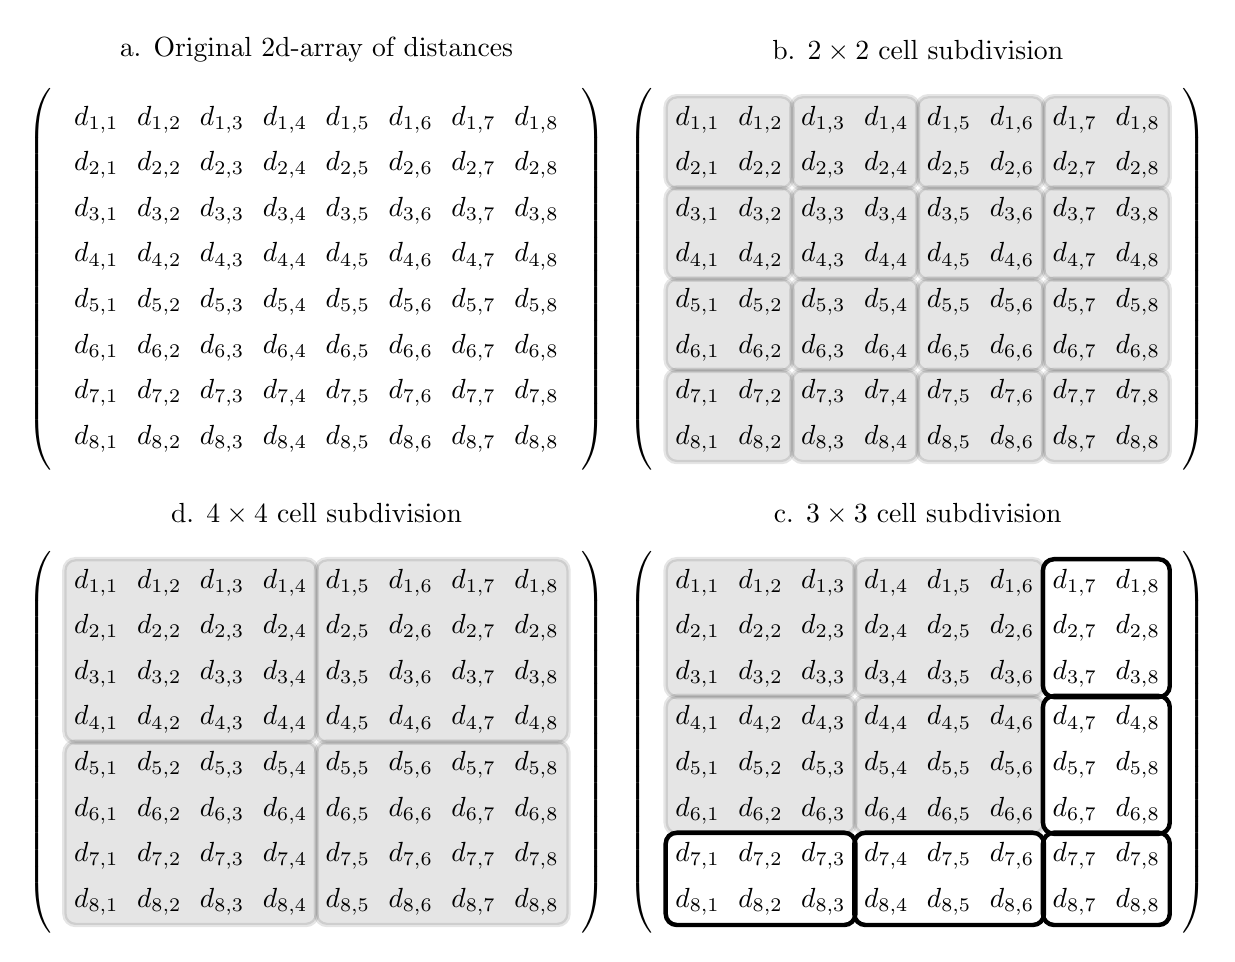
\begin{tikzpicture}
        \matrix [matrix of math nodes,left delimiter=(,right delimiter=)] (m0)
        {
            d_{1,1} & d_{1,2} & d_{1,3} & d_{1,4} & d_{1,5} & d_{1,6} & d_{1,7} & d_{1,8} \\ 
            d_{2,1} & d_{2,2} & d_{2,3} & d_{2,4} & d_{2,5} & d_{2,6} & d_{2,7} & d_{2,8} \\ 
            d_{3,1} & d_{3,2} & d_{3,3} & d_{3,4} & d_{3,5} & d_{3,6} & d_{3,7} & d_{3,8} \\ 
            d_{4,1} & d_{4,2} & d_{4,3} & d_{4,4} & d_{4,5} & d_{4,6} & d_{4,7} & d_{4,8} \\ 
            d_{5,1} & d_{5,2} & d_{5,3} & d_{5,4} & d_{5,5} & d_{5,6} & d_{5,7} & d_{5,8} \\ 
            d_{6,1} & d_{6,2} & d_{6,3} & d_{6,4} & d_{6,5} & d_{6,6} & d_{6,7} & d_{6,8} \\ 
            d_{7,1} & d_{7,2} & d_{7,3} & d_{7,4} & d_{7,5} & d_{7,6} & d_{7,7} & d_{7,8} \\ 
            d_{8,1} & d_{8,2} & d_{8,3} & d_{8,4} & d_{8,5} & d_{8,6} & d_{8,7} & d_{8,8} \\ 
        };
        
        \matrix [matrix of math nodes,left delimiter=(,right delimiter=),below=of m0] (m4)
        {
            d_{1,1} & d_{1,2} & d_{1,3} & d_{1,4} & d_{1,5} & d_{1,6} & d_{1,7} & d_{1,8} \\ 
            d_{2,1} & d_{2,2} & d_{2,3} & d_{2,4} & d_{2,5} & d_{2,6} & d_{2,7} & d_{2,8} \\ 
            d_{3,1} & d_{3,2} & d_{3,3} & d_{3,4} & d_{3,5} & d_{3,6} & d_{3,7} & d_{3,8} \\ 
            d_{4,1} & d_{4,2} & d_{4,3} & d_{4,4} & d_{4,5} & d_{4,6} & d_{4,7} & d_{4,8} \\ 
            d_{5,1} & d_{5,2} & d_{5,3} & d_{5,4} & d_{5,5} & d_{5,6} & d_{5,7} & d_{5,8} \\ 
            d_{6,1} & d_{6,2} & d_{6,3} & d_{6,4} & d_{6,5} & d_{6,6} & d_{6,7} & d_{6,8} \\ 
            d_{7,1} & d_{7,2} & d_{7,3} & d_{7,4} & d_{7,5} & d_{7,6} & d_{7,7} & d_{7,8} \\ 
            d_{8,1} & d_{8,2} & d_{8,3} & d_{8,4} & d_{8,5} & d_{8,6} & d_{8,7} & d_{8,8} \\ 
        };
        \draw[rounded corners,ultra thick, draw=black, fill=black, opacity=0.1] (m4-4-1.south west) rectangle (m4-1-4.north east);
        \draw[rounded corners,ultra thick, draw=black, fill=black, opacity=0.1] (m4-4-5.south west) rectangle (m4-1-8.north east);
        \draw[rounded corners,ultra thick, draw=black, fill=black, opacity=0.1] (m4-8-1.south west) rectangle (m4-5-4.north east);
        \draw[rounded corners,ultra thick, draw=black, fill=black, opacity=0.1] (m4-8-5.south west) rectangle (m4-5-8.north east);

        \matrix [matrix of math nodes,left delimiter=(,right delimiter=),right=of m4] (m3)
        {
            d_{1,1} & d_{1,2} & d_{1,3} & d_{1,4} & d_{1,5} & d_{1,6} & d_{1,7} & d_{1,8} \\ 
            d_{2,1} & d_{2,2} & d_{2,3} & d_{2,4} & d_{2,5} & d_{2,6} & d_{2,7} & d_{2,8} \\ 
            d_{3,1} & d_{3,2} & d_{3,3} & d_{3,4} & d_{3,5} & d_{3,6} & d_{3,7} & d_{3,8} \\ 
            d_{4,1} & d_{4,2} & d_{4,3} & d_{4,4} & d_{4,5} & d_{4,6} & d_{4,7} & d_{4,8} \\ 
            d_{5,1} & d_{5,2} & d_{5,3} & d_{5,4} & d_{5,5} & d_{5,6} & d_{5,7} & d_{5,8} \\ 
            d_{6,1} & d_{6,2} & d_{6,3} & d_{6,4} & d_{6,5} & d_{6,6} & d_{6,7} & d_{6,8} \\ 
            d_{7,1} & d_{7,2} & d_{7,3} & d_{7,4} & d_{7,5} & d_{7,6} & d_{7,7} & d_{7,8} \\ 
            d_{8,1} & d_{8,2} & d_{8,3} & d_{8,4} & d_{8,5} & d_{8,6} & d_{8,7} & d_{8,8} \\ 
        };
        \draw[rounded corners,ultra thick, draw=black, fill=black, opacity=0.1] (m3-3-1.south west) rectangle (m3-1-3.north east);
        \draw[rounded corners,ultra thick, draw=black, fill=black, opacity=0.1] (m3-3-4.south west) rectangle (m3-1-6.north east);
        \draw[rounded corners,ultra thick, draw=black,] (m3-3-7.south west) rectangle (m3-1-8.north east);
        \draw[rounded corners,ultra thick, draw=black, fill=black, opacity=0.1] (m3-6-1.south west) rectangle (m3-4-3.north east);
        \draw[rounded corners,ultra thick, draw=black, fill=black, opacity=0.1] (m3-6-4.south west) rectangle (m3-4-6.north east);
        \draw[rounded corners,ultra thick, draw=black] (m3-6-7.south west) rectangle (m3-4-8.north east);
        \draw[rounded corners,ultra thick, draw=black] (m3-8-1.south west) rectangle (m3-7-3.north east);
        \draw[rounded corners,ultra thick, draw=black] (m3-8-4.south west) rectangle (m3-7-6.north east);
        \draw[rounded corners,ultra thick, draw=black] (m3-8-7.south west) rectangle (m3-7-8.north east);


        \matrix [matrix of math nodes,left delimiter=(,right delimiter=), right= of m0] (m2)
        {
            d_{1,1} & d_{1,2} & d_{1,3} & d_{1,4} & d_{1,5} & d_{1,6} & d_{1,7} & d_{1,8} \\ 
            d_{2,1} & d_{2,2} & d_{2,3} & d_{2,4} & d_{2,5} & d_{2,6} & d_{2,7} & d_{2,8} \\ 
            d_{3,1} & d_{3,2} & d_{3,3} & d_{3,4} & d_{3,5} & d_{3,6} & d_{3,7} & d_{3,8} \\ 
            d_{4,1} & d_{4,2} & d_{4,3} & d_{4,4} & d_{4,5} & d_{4,6} & d_{4,7} & d_{4,8} \\ 
            d_{5,1} & d_{5,2} & d_{5,3} & d_{5,4} & d_{5,5} & d_{5,6} & d_{5,7} & d_{5,8} \\ 
            d_{6,1} & d_{6,2} & d_{6,3} & d_{6,4} & d_{6,5} & d_{6,6} & d_{6,7} & d_{6,8} \\ 
            d_{7,1} & d_{7,2} & d_{7,3} & d_{7,4} & d_{7,5} & d_{7,6} & d_{7,7} & d_{7,8} \\ 
            d_{8,1} & d_{8,2} & d_{8,3} & d_{8,4} & d_{8,5} & d_{8,6} & d_{8,7} & d_{8,8} \\ 
        };
        \draw[rounded corners,ultra thick, draw=black, fill=black, opacity=0.1] (m2-2-1.south west) rectangle (m2-1-2.north east);
        \draw[rounded corners,ultra thick, draw=black, fill=black, opacity=0.1] (m2-2-3.south west) rectangle (m2-1-4.north east);
        \draw[rounded corners,ultra thick, draw=black, fill=black, opacity=0.1] (m2-2-5.south west) rectangle (m2-1-6.north east);
        \draw[rounded corners,ultra thick, draw=black, fill=black, opacity=0.1] (m2-2-7.south west) rectangle (m2-1-8.north east);
        \draw[rounded corners,ultra thick, draw=black, fill=black, opacity=0.1] (m2-4-1.south west) rectangle (m2-3-2.north east);
        \draw[rounded corners,ultra thick, draw=black, fill=black, opacity=0.1] (m2-4-3.south west) rectangle (m2-3-4.north east);
        \draw[rounded corners,ultra thick, draw=black, fill=black, opacity=0.1] (m2-4-5.south west) rectangle (m2-3-6.north east);
        \draw[rounded corners,ultra thick, draw=black, fill=black, opacity=0.1] (m2-4-7.south west) rectangle (m2-3-8.north east);
        \draw[rounded corners,ultra thick, draw=black, fill=black, opacity=0.1] (m2-6-1.south west) rectangle (m2-5-2.north east);
        \draw[rounded corners,ultra thick, draw=black, fill=black, opacity=0.1] (m2-6-3.south west) rectangle (m2-5-4.north east);
        \draw[rounded corners,ultra thick, draw=black, fill=black, opacity=0.1] (m2-6-5.south west) rectangle (m2-5-6.north east);
        \draw[rounded corners,ultra thick, draw=black, fill=black, opacity=0.1] (m2-6-7.south west) rectangle (m2-5-8.north east);
        \draw[rounded corners,ultra thick, draw=black, fill=black, opacity=0.1] (m2-8-1.south west) rectangle (m2-7-2.north east);
        \draw[rounded corners,ultra thick, draw=black, fill=black, opacity=0.1] (m2-8-3.south west) rectangle (m2-7-4.north east);
        \draw[rounded corners,ultra thick, draw=black, fill=black, opacity=0.1] (m2-8-5.south west) rectangle (m2-7-6.north east);
        \draw[rounded corners,ultra thick, draw=black, fill=black, opacity=0.1] (m2-8-7.south west) rectangle (m2-7-8.north east);
        \node[above= 0.2cm of m0] {a. Original 2d-array of distances};
        \node[above= 0.2cm of m2] {b. $2 \times 2$ cell subdivision};
        \node[above= 0.2cm of m3] {c. $3 \times 3$ cell subdivision};
        \node[above= 0.2cm of m4] {d. $4 \times 4$ cell subdivision};
    \end{tikzpicture}